\section{Konzept}
\label{sec:concept}

In den vorangegangenen Kapiteln wurde zusammengefasst, was die Dateiverwaltung der Schul-Cloud leisten muss und woran sie sich orientieren kann. Vom Partner des Bachelor-Projekts MINT-EC \footnote{Verein mathematisch-naturwissenschaftlicher Excellence-Center an Schulen e. V. (MINT-EC) - \url{https://www.mint-ec.de/}}  und dem Hasso-Plattner-Institut wurde eine Anforderungsspezifikation erstellt, an welcher sich das folgende Konzept der Dateiverwaltung orientiert (Abbildung 2). Neben der Verwaltung von eigenen Dateien, sollen auch  jene im Kurs- bzw. Fächer- so wie Klassenkontext verteilbar sein. Dies soll dazu dienen, digitale Inhalte besser in den Unterricht einzubetten und (Haus)-Aufgaben mithilfe von anschaulichem Material zu gestalten. Somit sollen diese Dateien über eine einheitliche Schnittstelle durch die Backend-API sowie über das Web-Frontend in mehreren Kontexten verfügbar sein. Außerdem soll es für eine Schule möglich sein, eine bereits bestehende Dateiablage einzubinden. 

\begin{figure}[H]
	\centering
	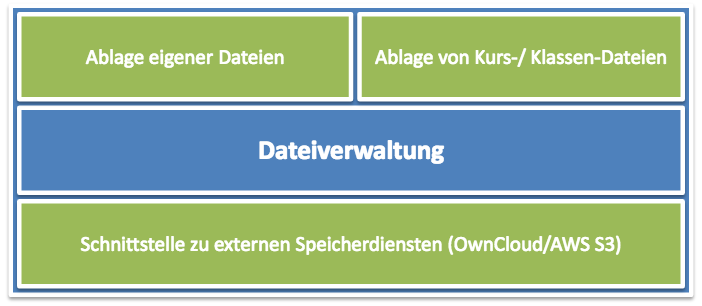
\includegraphics[width=0.8\linewidth]{images/AnforderungenDateiverwaltung}
	\caption[Caption for concept]{Grundanforderungen an die Dateiverwaltung der Schul-Cloud\footnotemark}
\end{figure}
\footnotetext{Martin Hense (Mint-EC - \url{https://www.mint-ec.de/})}


\subsection{Grundaufbau Dateiverwaltung}

Die grundlegende Struktur sieht vor, dass jede Schule seine eigene logische Einheit besitzt. Diese wird im folgenden \textit{Bucket} genant und leitet sich vom AWS S3 Standart ab (Abschnitt 2.3.1). Das dient zum einen der besseren Organisation innerhalb der Schul-Cloud, da Nutzer im Datenmodell zu einer Schule zusammengefasst werden. Außerdem folgt das Projekt dem Prinzip \textit{Privacy by Design} \footnote{Privacy by Design - \url{https://digitalcourage.de/blog/2015/was-ist-privacy-design} }. Damit wird sichergestellt, dass eine Schule außerhalb von anderen Schulen modular abgekapselt ist. Somit ist von vornherein  eine Sicherheit der Dateien auf Schulebene gewährleistet. Diese Schul-Buckets können auf getrennten Servern liegen, so dass zum Beispiel eine Schule aus Niedersachsen auf eine eigene ownCloud zurückgreifen kann und eine Schule aus Hamburg einen S3-Provider benutzen kann. Das Prinzip des \textit{File Sharing} (Abschnitt 3.4.) kann diese logische Abkapselung ein wenig aufbrechen, um Dateien auch über Schulebene hinaus teilbar zu machen. Eine Erweiterung von Buckets auf Landkreis - oder Bundeslandebene erscheint als weitere Option. Jedoch wird sich diese Arbeit auf die Einteilung in Schul-Buckets beschränken. Dieses Konzept ist aber ohne weiteres skalierbar auf größere Kontexte.  Die Abbildung 3 zeigt im folgenden die weitere Unterteilung eines Buckets. Dieser wird in vier Teilkomponenten innerhalb der Schule  untergliedert. Wenn ein Bucket als einer Art Oberordner oder Root-Verzeichnis verstanden werden kann, dann sind diese Teilkomponenten schlichtweg Unterordner des Buckets. Zum einen gibt es den Ordner \textit{courses}, dieser enthält alle Dateien, welche zu Kursen bzw. Fächer gehören. Für eine bessere Unterteilung befinden sich hier sehr viele Unterordner, welche bloß die \textit{courseId} eines Schul-Cloud-Kurses referenzieren. Dies dient der Verteilung aller Kurs-Dateien zu dem zugehörigen Kurs. Diese ID-Ordnernamen werden von Schul-Cloud-Server versteckt und nicht im User Interface des Schul-Cloud-Clients angezeigt. So hat man aber zum Beispiel die Möglichkeit, über die \textit{courseId} alle Dateien eines Kurses zu erhalten. Auf diese haben nur Lehrer und Schüler des Kurses bzw. Faches Zugriff. Die Berechtigungsverwaltung übernimmt der Schul-Cloud-Server und wird in der Implementierung (Abschnitt 4.1.2) genauer beschrieben. \\

Ähnlich wie der \textit{courses} Unterordner gibt es den \textit{classes} und \textit{users} Unterordner. Beim ersten werden im gleichen Schema alle Dateien von Schul-Cloud Klassen verteilt, wieder referenziert über den jeweiligen ID-Unterordner. Zugriff haben hier nur Lehrer und Schüler der Klasse. Der \textit{users} Unterordner bildet die persönlichen Dateien eines jeden Nutzers der Schule, egal ob Lehrer, Schüler oder Administrator. Als Zusatz für schulübergreifende Dateien gibt es den Unterordner \textit{school}. Schreibrechte hat hier nur der Administrator der Schule, zugreifen kann jedoch jeder Nutzer der Schule. Natürlich kann es nun vorkommen, dass eine Schule bereits eine ausgeprägte Dateistruktur besitzt und der Grundaufbau mit den vier Unterkomponenten nicht abbildbar sein könnte. Hier muss der Schul-Cloud-Server dafür sorgen, dass diese Dateien trotzdem über die Schul-Cloud zugänglich sind. Eine Möglichkeit wäre es, dass die gesamte Struktur zu Beginn in den \textit{schools} Ordner gelegt wird und diese von dahin auf die jeweiligen Kontexte verlegt werden.

\begin{figure}[H]
	\centering
	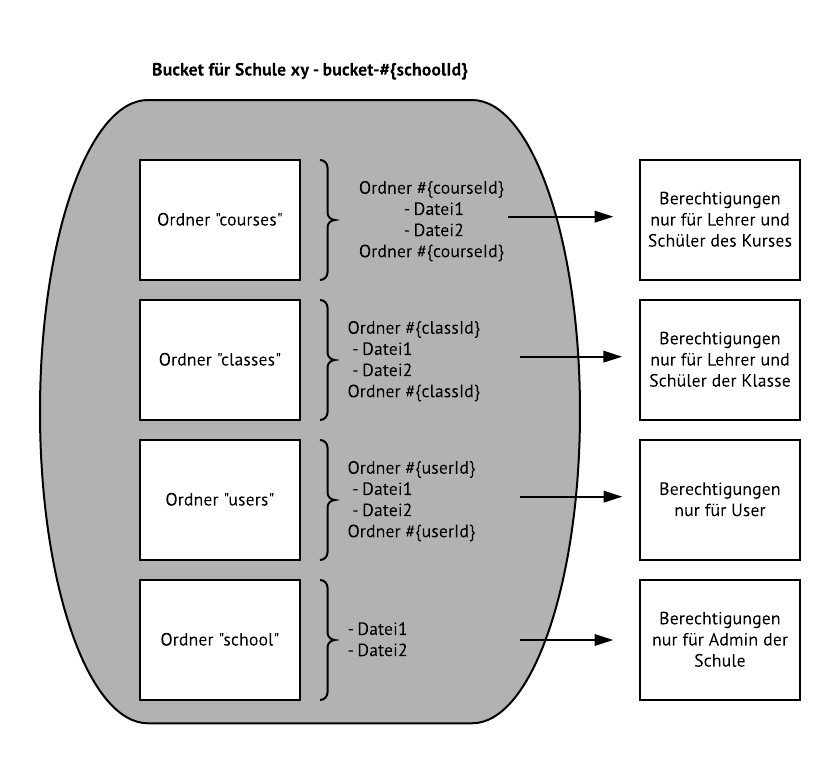
\includegraphics[width=0.8\linewidth]{images/AufbauDateiverwaltung}
	\caption[Caption for concept]{Grundaufbau eines Schul-Buckets}
\end{figure}

\subsection{Architektur verteilter Provider}

Die Schul-Cloud stellt während der Pilotphase zwar nur eine S3-Instanz \footnote{Technischer Bericht der Schul-Cloud, Seite 39 \cite{paper:technischerbericht}}, worüber die Buckets der Pilotschulen liegen. Trotzdem soll es die Architektur der Dateiverwaltung möglich machen, Buckets auch auf mehrere Server zu verteilen. Dafür macht sich der Server das Strategy-Pattern \footnote{Strategy-Pattern - \url{https://de.wikipedia.org/wiki/Strategie_(Entwurfsmuster)}} zu Nutze. Dieses sieht vor, dass eine abstrakte Strategie die Schnittstellen vorgibt und mehrere Strategien diese implementieren. In Form dieser können so Anbindungen an verschiedene Typen von File Storage Providern erstellt werden. In der Implementierung wird eine solche Strategie am Beispiel von AWS S3 (Abschnitt 4.1.3) geschildert. Abbildung 4 zeigt die Verteilung der verschiedenen File Storage Strategien. So ist es möglich, über den Schul-Kontext, der die Art des Provider bestimmt, die richtige Strategie zu bestimmen und auf die Schuldateien zugreifen zu können. Diese Aufteilung macht die Verteilung von Buckets auf mehrere Server ausführbar. So kann ein Bucket auf einer S3-Instanz liegen und mittels S3-Strategie darauf zugegriffen werden, sowie eine ownCloud-Instanz durch die ownCloud-Strategie auf einem anderen Server. 

\todo{Alternative, falls Bucket von vornherein nicht den Standardaufbau besitzt}

\begin{figure}[H]
	\centering
	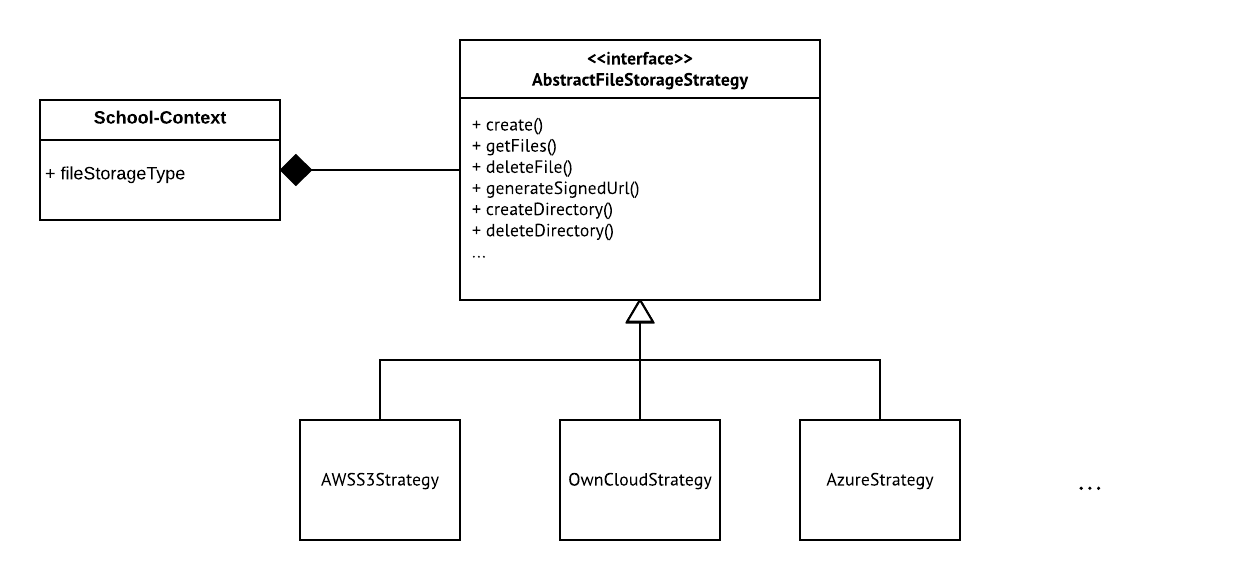
\includegraphics[width=1\linewidth]{images/strategypattern}
	\caption[Caption for concept]{Verteilung der Schul-Buckets mithilfe des Strategy-Patterns}
\end{figure}

\subsection{Interaktion verschiedener Schul-Cloud Komponenten}

\todo{Bilder Qualität verbessern!!}

\begin{figure}[H]
	\centering
	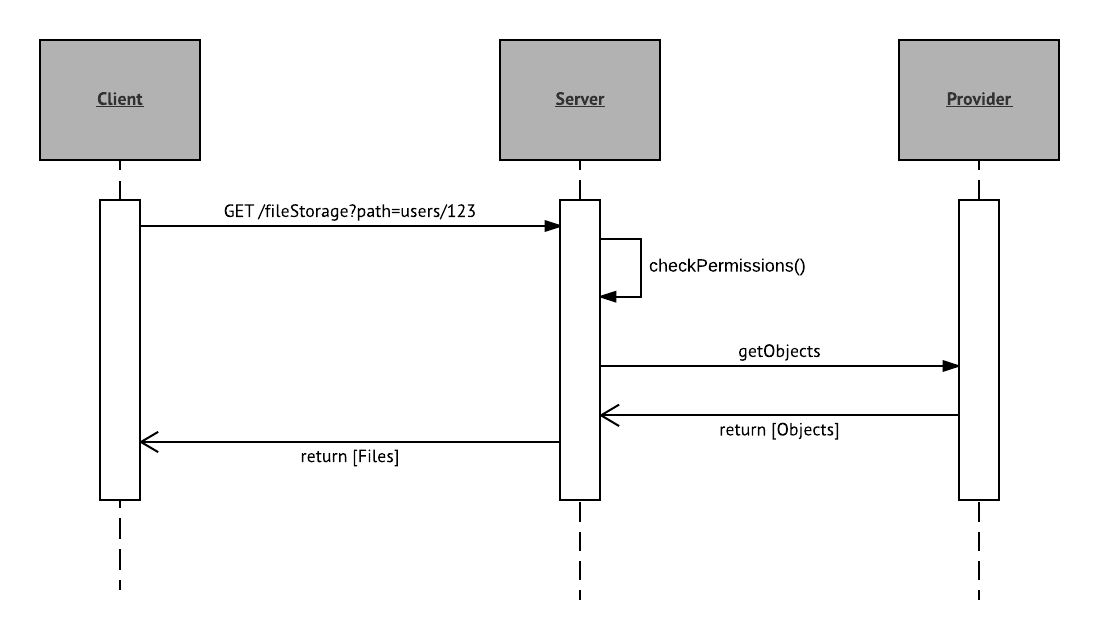
\includegraphics[width=1\linewidth]{images/fileumlsequence}
	\caption[Caption for concept]{Interaktion zwischen Client, Server und File Storage Provider}
\end{figure}


\subsection{Teilen von Dateien}

\begin{figure}[H]
	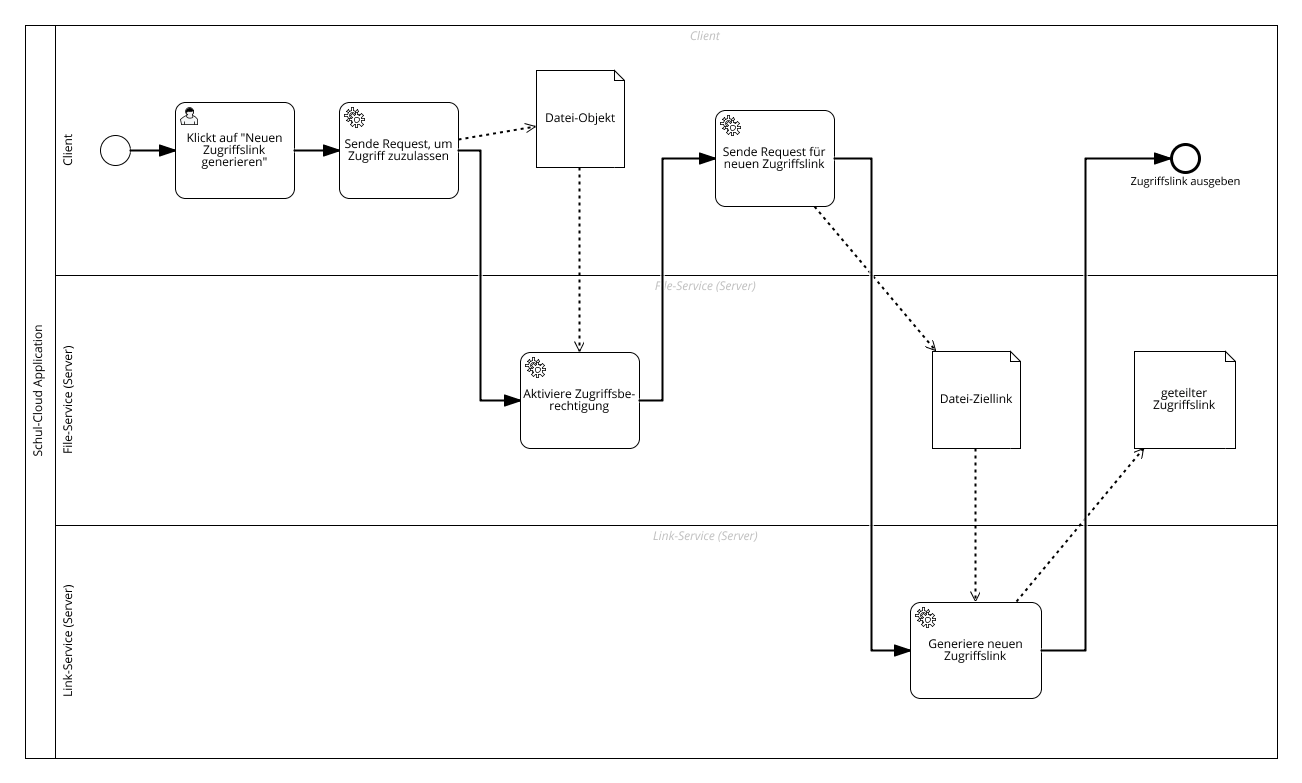
\includegraphics[width=1\linewidth]{images/filesharinggeneration}
	\caption[Caption for concept]{Generierung eines Zugriffslinks}
	\centering
\end{figure}

\begin{figure}[H]
	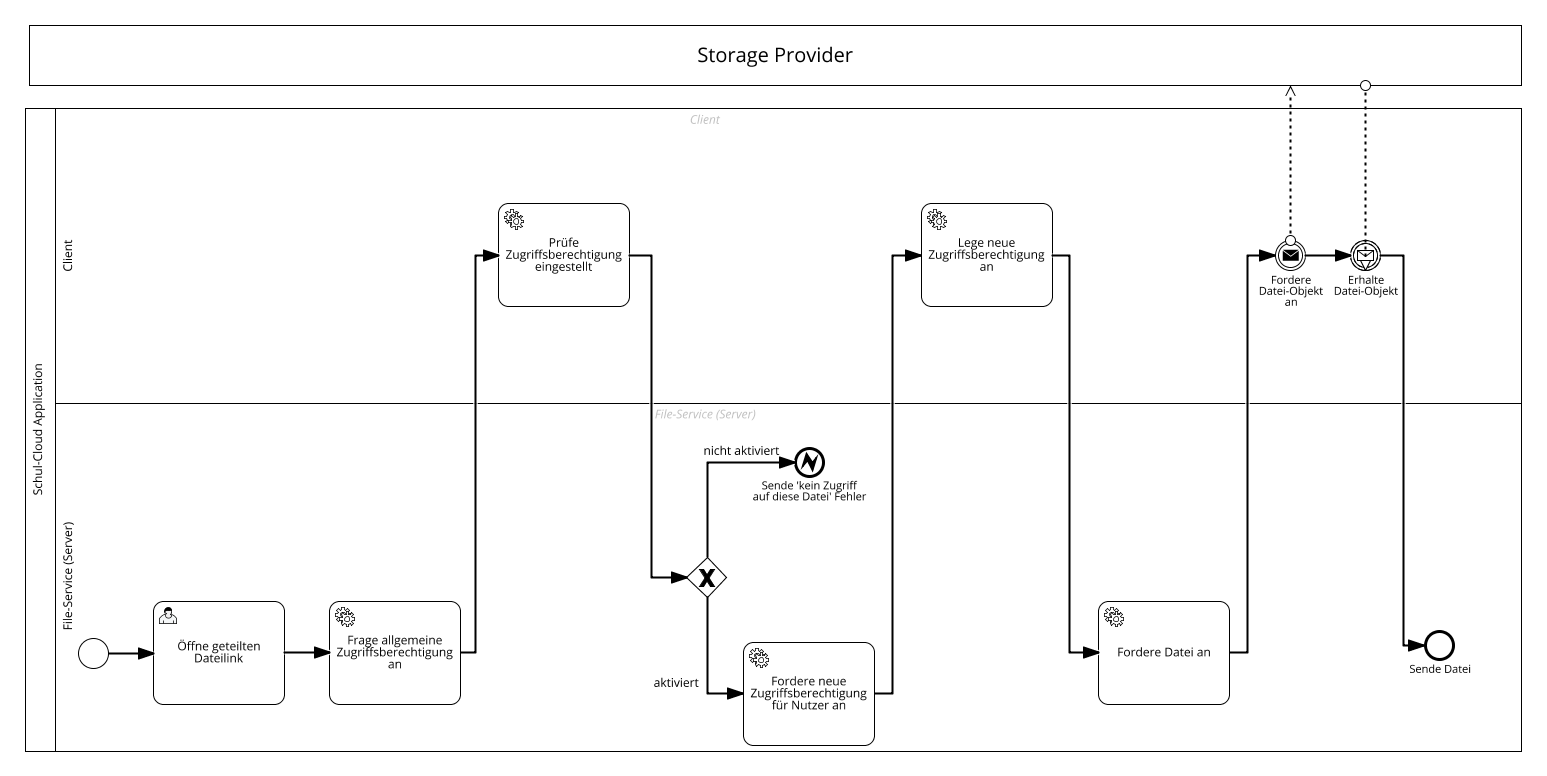
\includegraphics[width=1\linewidth]{images/filesharingusing}
	\caption[Caption for concept]{Zugriff auf eine geteilte Datei}
	\centering
\end{figure}


\clearpage
